\documentclass[a4paper,10pt]{report}
\usepackage{url}
\usepackage{breakurl} 
\usepackage[breaklinks]{hyperref}
\usepackage[utf8]{inputenc}
\usepackage[T1]{fontenc}
\usepackage[polutonikogreek, polish]{babel}
\usepackage{indentfirst}
\usepackage{polski}
\usepackage{listings}
\usepackage{mdframed}
\usepackage{graphicx}
\usepackage{fancyhdr}
\usepackage{pdfpages}
\usepackage{hyperref}
\usepackage{tabularx} 
\usepackage{pdfpages}
\usepackage{amsthm}
\usepackage{color}
\definecolor{lightgray}{rgb}{.9,.9,.9}
\definecolor{darkgray}{rgb}{.4,.4,.4}
\definecolor{purple}{rgb}{0.65, 0.12, 0.82}
\lstdefinestyle{sharpc}{language=[Sharp]C}
\lstdefinelanguage{JavaScript}{
	keywords={break, case, catch, continue, debugger, default, delete, do, else, false, finally, for, function, if, in, instanceof, new, null, return, switch, this, throw, true, try, typeof, var, void, while, with},
	morecomment=[l]{//},
	morecomment=[s]{/*}{*/},
	morestring=[b]',
	morestring=[b]",
	ndkeywords={class, export, boolean, throw, implements, import, this},
	keywordstyle=\color{blue}\bfseries,
	ndkeywordstyle=\color{darkgray}\bfseries,
	identifierstyle=\color{black},
	commentstyle=\color{purple}\ttfamily,
	stringstyle=\color{red}\ttfamily,
	sensitive=true
}

\lstdefinelanguage{cpp}{
	keywords={auto, struct, int, double, class, template, typename, break, case, catch, continue, debugger, default, delete, do, else, false, finally, for, function, if, in, instanceof, new, null, return, switch, this, throw, true, try, typeof, var, void, while, with, decltype, namespace, public, private, protected},
	morecomment=[l]{//},
	morecomment=[s]{/*}{*/},
	morestring=[b]',
	morestring=[b]",
	ndkeywords={class, export, boolean, throw, implements, import, this},
	keywordstyle=\color{blue}\bfseries,
	ndkeywordstyle=\color{darkgray}\bfseries,
	identifierstyle=\color{black},
	commentstyle=\color{purple}\ttfamily,
	stringstyle=\color{red}\ttfamily,
	sensitive=true
}

\lstset
{ %Formatting for code in appendix
	language=Java,
	basicstyle=\footnotesize,
	numbers=left,
	stepnumber=1,
	showstringspaces=false,
	tabsize=1,
	breaklines=true,
	breakatwhitespace=false,
}
\newmdtheoremenv{theo}{Definicja}
\frenchspacing
\emergencystretch=1em

%opening
\title{API funkcyjne w języku C++}
\author{Krzysztof Osiecki}
\begin{document}\pagestyle{fancy}\lhead{}\rightmark
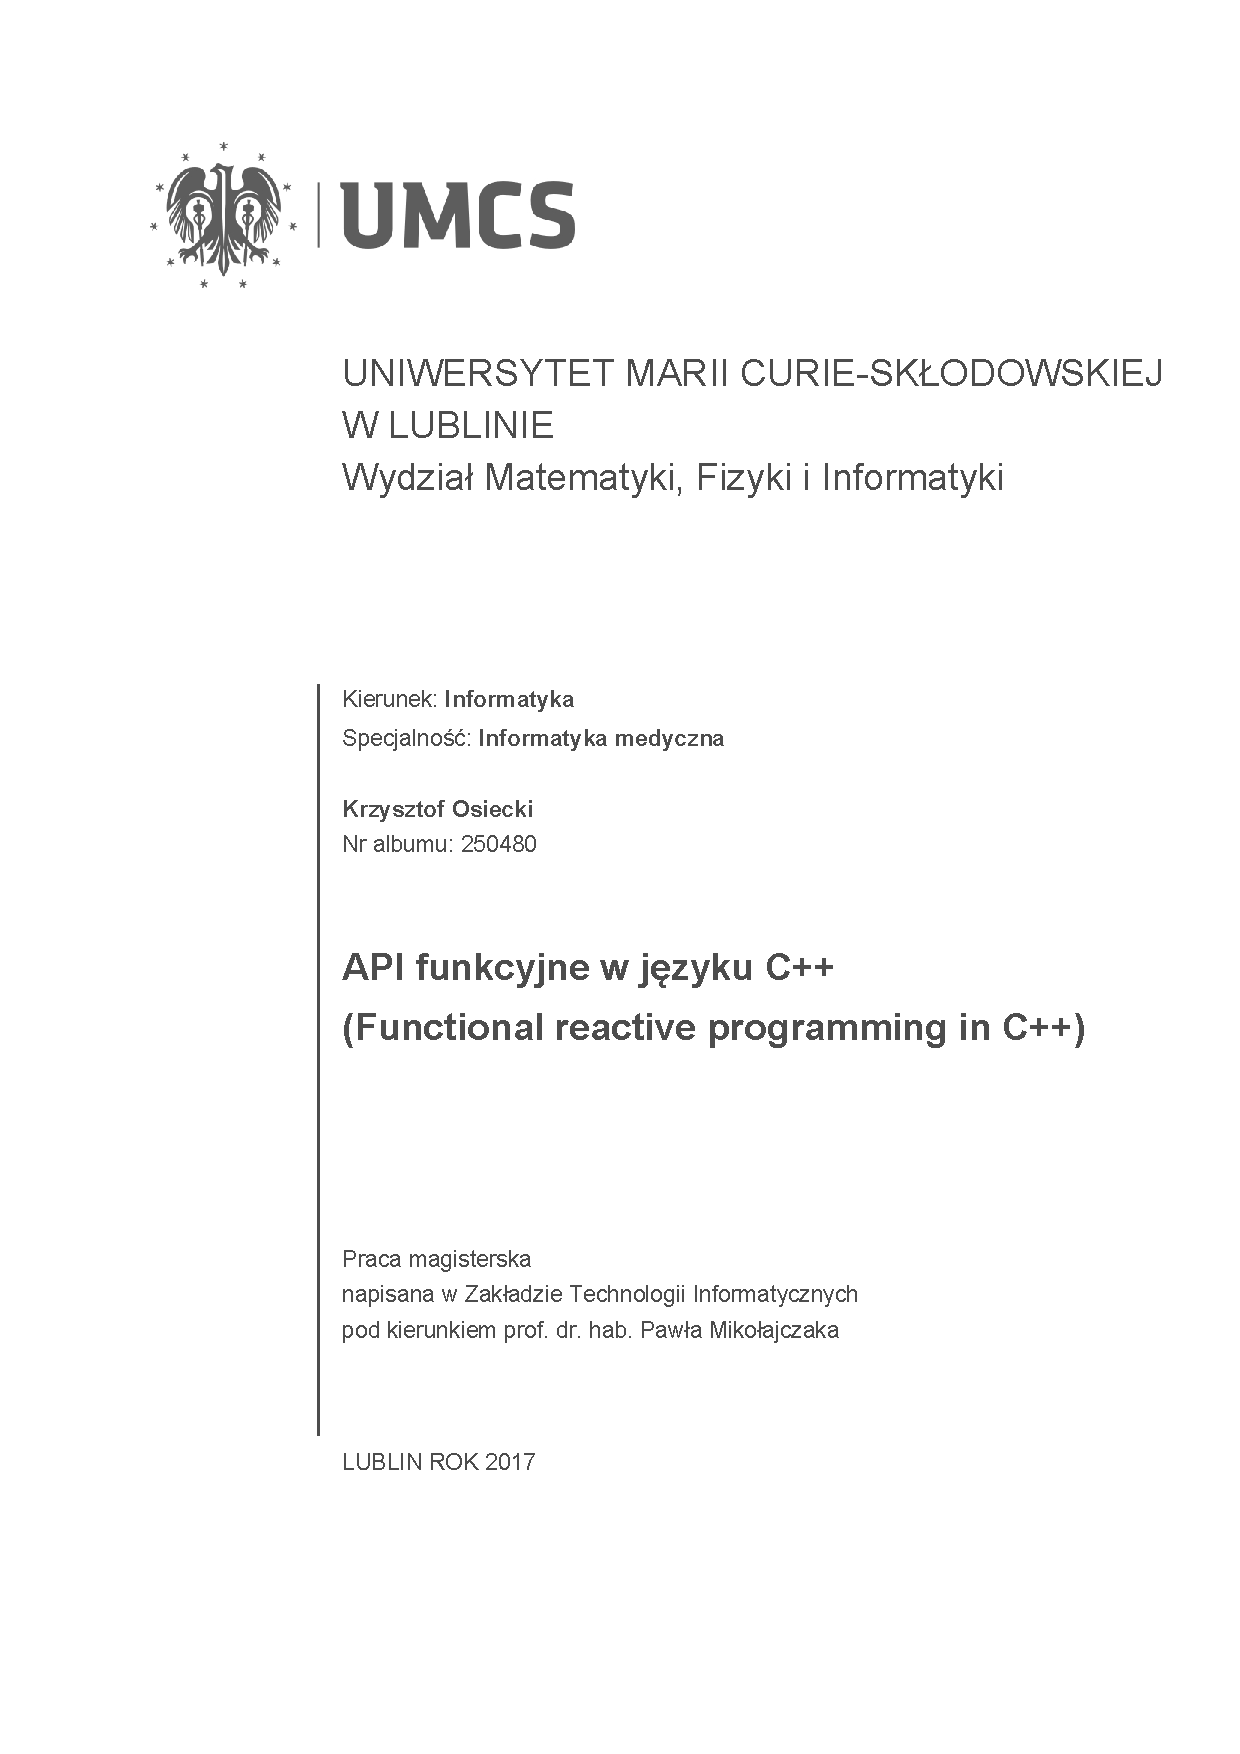
\includepdf{tytul.pdf}
\tableofcontents{}
\chapter*{Wstęp}
Programowanie samo w sobie jest procesem mającym na celu stworzenie działającego oprogramowania. W celu wykonania całego tego procesu podejmuje się wiele działań. Etapami procesu programowania są: projektowanie, testowanie i utrzymanie kodu, a także przede wszystkim to co może być przez niektórych utożsamiane z programowaniem, czyli pisanie kodu programów. Obecnie dąży się do strukturalizowania każdego z tych etapów. Powstały różne metodyki oraz modele, mające ułatwić zarządzanie wytwarzaniem oprogramowania. Są one różne w zależności od skali projektów, terminów czy stopnia wydajności, bądź zdolności do podejmowania autonomicznych decyzji przez programistów. U podstaw każdej z metodyk leży ostatecznie kod programu. Kod, który może być napisany na wiele sposobów w wielu językach programowania. Podobnie jak w przypadku metodyk, języki różnią się między sobą stopniem dopasowania do konkretnych rozwiązań. Niniejsza praca przedstawia ogólny podział języków programowania, ze względu na podejście do tworzenia kodu, skupiając się głównie na podejściu funkcyjnym. W pierwszym rozdziale zostaną przedstawione ogólne koncepcje, które pozwalają na funkcyjne tworzenie kodu niezależnie od języka. Rozdział drugi ma na celu porównanie dwóch głównych paradygmatów programowania oraz prezentacje zalet paradygmatu funkcyjnego. W rozdziale trzecim, opisane zostały gotowe rozwiązania, zaimplementowane w różnych językach pozwalające, na funkcyjną obsługę kolekcji, oraz posługiwania się funkcjami jako obiektami domknięcia. Ostatni rozdział przedstawia przygotowane API. API z języka angielskiego \verb|Aplication Programing Interface|, czyli interfejs programowania aplikacji, oznacza zbiór funkcji oferowanych w tym przypadku w postaci biblioteki do języka \verb|C++|. Przygotowane rozwiązanie ma umożliwić funkcyjną obsługę kolekcji w języku \verb|C++|. 
\chapter{Omówienie funkcyjnego paradygmatu programowania}
\section{Czym jest paradygmat programowania}
\paragraph{}
Wspomniana we wstępie kategoria podejścia do tworzenia programów określana jest mianem paradygmatu programowania.
\begin{theo}
	Paradygmat - przyjęty sposób widzenia rzeczywistości w danej dziedzinie, doktrynie.
\end{theo}
 Paradygmat nie jest określany przez język programowania, lecz przez sposób w jaki programista opisuje problem, który rozwiązuje. Paradygmaty w dziedzinie programowania podzielić można na dwie główne grupy. Paradygmat imperatywny oraz deklaratywny. W paradygmacie imperatywnym, motywem przewodnim programu jest instrukcja. Instrukcja stanowi rozkaz dla procesora, zaś program składa się z wykonania odpowiedniej ilości takich rozkazów. Jest to chyba najbardziej rozpowszechniona, kategoria programowania. Powodem takiego stanu rzeczy jest najprawdopodobniej fakt, iż języki imperatywne są tymi, od których w większości przypadków zaczyna się naukę programowania. Najpopularniejszymi językami akademickimi są \verb|C++| oraz \verb|Pascal|, które ze swej natury są imperatywne. Wydawać by się jednak mogło, że bliższy ludzkiemu sposobowi rozwiązywania problemów będzie podejście deklaratywne. W paradygmacie deklaratywnym program stanowi opis rozwiązania. Programista nie odpowiada, za instruowanie procesora jak ma wykonywać poszczególne czynności. Opisuje tylko spodziewany rezultat, a właściwie cechy tego rezultatu. Zadaniem komputera, a w zasadzie kompilatora, bądź interpretera, konkretnego języka jest odpowiednie dopasowanie działań w celu uzyskania odpowiednich rezultatów. Znanym powszechnie przykładem tego podejścia może być język \verb|SQL|. Zapytanie w tym języku polega na opisaniu, oczekiwanego wyniku. Na tej podstawie silnik bazy danych, wykonuje odpowiednie operacje. Piszący kwerendę nie musi wiedzieć w jakiej strukturze znajdują się dane, ani jak efektywnie się do nich dostać. 
 \paragraph{}
 W praktyce rzadko spotyka się języki w całości oparte tylko na jednym paradygmacie. Spowodowane jest to ograniczeniami, jakie musiałby być realizowane w celu pełnego spełnienia założeń, każdego z nich. Najczęściej okazuje się, że idealnym rozwiązaniem jest połączenie najlepszych cech każdego z nich. Obecnie większość popularnych języków programowania, jest językami wieloparadygmatowymi. Posiadają one zarówno cechy imperatywne jak i deklaratywne. Do tego wewnętrzny podział tych głównych grup powoduje jeszcze większe rozdrobnienie kategorii danego języka. Określenie paradygmat często występuje wymiennie ze słowem programowanie. Oznacza to, że pojęcia programowanie deklaratywne i paradygmat deklaratywny są tożsame, dlatego będą w niniejszej pracy stosowane wymiennie.
\section{Cechy paradygmatu funkcyjnego}
Programowanie funkcyjne jest odmianą programowania deklaratywnego. Główną cechą tego paradygmatu jest skupienie uwagi na funkcjach i obliczaniu ich wartości. W programowaniu funkcyjnym, funkcja zachowuje się tak samo jak funkcja matematyczna. To znaczy, że dla parametrów dla których jest poprawnie zdefiniowana, będzie zawsze zwracać tą samą wartość. Wykonanie programu polega zatem na obliczeniu wartości składających się na niego funkcji.
Ważną cechą funkcji w sensie matematycznym jest jej bezstanowość. Każda funkcja matematyczna posiada swoją definicję, która określa jej wynik w zależności od zadanych argumentów. Dla określonego zbioru argumentów funkcja zawsze zwróci ustaloną wartość. Niezależnie od czynników zewnętrznych ani ilości jej wywołań. Programowanie funkcyjne jako bazujące silnie na matematycznych podstawach, stara się emulować takie zachowanie funkcji. W programowaniu imperatywnym sytuacja wygląda inaczej. Można powiedzieć, że większą część programowania imperatywnego stanowi coś co określa się mianem \verb|efektów ubocznych|. Każde zachowanie funkcji (tutaj programistycznej, nie matematycznej) nie będące wyliczeniem i zwróceniem wartości nazywane jest efektem ubocznym. W przypadku imperatywnego programowania będą to na przykład: operacje obsługi wejścia/wyjścia, utworzenie zmiennej, czy obiektu w pamięci, modyfikacja struktury danych. Z funkcyjnego punktu widzenia, tego typu operacje są \verb|"brudne"| i nie pozwalają na zachowanie czystości języka funkcyjnego. Trudno jednak nie zauważyć jak wielkie znaczenie w świecie obecnego tworzenia oprogramowania odgrywa możliwość interakcji użytkownika z systemem. A skoro operacje wejścia/wyjścia nie są dozwolone w języku funkcyjnym, nie trudno się domyślić, że tego typu język raczej nie ma szans podbić komercyjnego rynku.
\section{Dlaczego paradygmat funkcyjny?}
Pomimo tej wady, paradygmat funkcyjny posiada cechy, które niewątpliwie stanowią jego ogromną zaletę. Sprawiły one, że nie został on zapomniany, a raczej powraca co jakiś czas w różnych formach i znajduje drogę do najpopularniejszych współcześnie języków. Przede wszystkim jako podzbiór paradygmatu deklaratywnego, programowanie funkcyjne nie wymaga od nas, konkretnego opisu działania, lecz opisu oczekiwanego przez nas wyniku. Dodatkowo potraktowanie funkcji jako \verb|obywatela pierwszej kategorii| sprawia, że normalnym staje się możliwość przekazania jednej funkcji jako parametru drugiej i wywołania jej kiedy będzie potrzebna, z argumentami, które w momencie jej tworzenia mogły być nie dostępne. Daje to w ręce programisty naprawdę potężne narzędzie, w przypadku aplikacji sterowanych zdarzeniowo. Na koniec zostawiam cechę, która sprawia, że w ogóle następują próby wplatania paradygmatu funkcyjnego do imperatywnych języków (przecież, imperatywnie i tak można te operacje wykonać). Cechą tą jest składnia, która w językach funkcyjnych jest niezwykle atrakcyjna dla programisty. Korzystając z funkcyjnych interfejsów, nie spotkamy kodu w którym przez piętnaście kolejnych linii definiujemy zmienne, po to żeby w szesnastej utworzyć z ich pomocą obiekt, a w siedemnastej wykonać na tym obiekcie jakąś metodę. Operacja sortowania w programowaniu funkcyjnym wymaga od nas kolekcji do posortowania i funkcji definiującej liniowy porządek na obiektach tej kolekcji. Jest to oczywiście tylko i wyłącznie kwestia odpowiednio wysokopoziomowego API. Jednak utworzenie go w sposób przyjazny dla użytkownika jest dużo łatwiejsze w językach, które paradygmat funkcyjny starają się adaptować, niż w tych, które zdecydowanie go odrzucają.
\section{Domknięcia i wyrażenia lambda jako sposób realizacji paradygmatu}
Jednym ze sposobów realizacji funkcyjnych aspektów w językach imperatywnych, są wyrażenia lambda. Wyrażenia te są w rzeczywistości, anonimowymi funkcjami, które można łatwo definiować i przekazywać jako parametry. Pojęcie lambd pozwoliło traktować je jako obiekty w językach w których funkcje, nie są domyślnie traktowane jako obiekty pierwszej kategorii. Najważniejszą ich cechą, która zapewnia ich użyteczność jest łatwość ich definiowania. Lambdę można zdefiniować w miejscu w którym jest potrzebna i przekazać od razu do wykonania innej funkcji, bądź jeśli istnieje potrzeba ponownego użycia, przypisać do zmiennej i wykorzystywać wielokrotnie. Od strony formalnej, lambdy stanowią konkretną implementację koncepcji domknięcia.
\begin{theo}
Domknięcie – w metodach realizacji języków programowania jest to obiekt wiążący funkcję lub referencję do funkcji oraz środowisko mające wpływ na tę funkcję w momencie jej definiowania.
\end{theo}
Domknięcie stanowi więc pojęcie szersze, którym można określić wszystkie implementacje pozwalające na użycie funkcji w kontekście obiektu, w paradygmacie programowania obiektowego.
\section{Kolekcje jako strumienie danych}
Wszystkie kolekcje, można przy przyjęciu odpowiedniego poziomu abstrakcji traktować jako strumień danych. Zarówno listy jak i drzewa, poza faktem, zapewnienia struktury, dla danych w której łatwo można nimi zarządzać, stanowią często źródło, które należy zużyć. Oczywiście kolejność iteracji po poszczególnych elementach może być różna, różne może być także podejście do konieczności przejścia po wszystkich elementach. Kluczową jednak cechą jest chęć wykonania pewnej operacji na całym, bądź przefiltrowanym w jakiś sposób zbiorze danych. Podejście takie i korzyści, które z niego płynął, są główną przyczyną powstania niniejszej pracy. Tego typu rozwiązania, zaimplementowano już w wielu językach programowania. W następnych podrozdziałach przestawiono, sposoby implementacji tych rozwiązań.
\chapter{Zalety programowania funkcyjnego w rozwiązaniach praktycznych}
\section{Podstawowe problemy i zadania w programowaniu aplikacji biznesowych}
Biznes wymaga oprogramowania. Ta kwestia nie podlega wątpliwości. Aplikacje bankowe, kasy w sklepach, giełda czy obecnie nawet telefony menadżerów, wszystkie te urządzenia i dziedziny wymagają odpowiednich programów pozwalających im wykonywać określone zadania. Popularność technologii informatycznych sprawia, że w zasadzie każda firma chcąca się rozwijać musi z tychże technologii korzystać. Czy to tworząc stronę internetową, czy monitorując pracowników, zarządzając urlopami czy katalogując zamówienia. O ile istnieją oczywiście sektory, w których od programisty wymaga się algorytmicznego myślenia, takie jak rynek procesorów, kart graficznych, badania naukowe czy związana blisko z biznesem kryptografia, to doświadczenie autora pozwala twierdzić, że większość informatyków znajdzie zatrudnienie przy znacznie mniej wymagających zadaniach. Poziom mocy obliczeniowej obecnych komputerów pozwala nam w wielu przypadkach nie przejmować się złożonością obliczeniową czy pamięciową podejmowanych przez programy działań (oczywiście w granicach rozsądku). Do tego z poziomu biznesu, oprogramowanie jest niczym innym jak tylko kosztem. Kosztem uzasadnionym z którym się pogodzono, ale jednak kosztem. A koszta należy minimalizować, dlatego jeśli menadżer projektu stanie przed wyborem pozostawienia programisty zarabiającego pięć tysięcy złotych na miesiąc z problemem optymalizacji algorytmu, albo zakupienia szybszego procesora z trzy tysiące złotych, z radością kupi procesor i przypisze sobie zasługi oszczędzenia dwóch tysięcy. Oczywiście gdyby tego typu problemy były częste, należałby szukać programisty, który na tego typu zadanie będzie potrzebował tydzień zamiast miesiąca. Jednak w codziennej pracy tego typu problemy prawie nie występują. Deweloperzy produkują prawie seryjnie aplikacje, które z ich punktu widzenia niczym się od siebie nie różnią. Implementacja sklepu internetowego sprzedającego traktory i sklepu sprzedającego koszule, są tym samym zadaniem. Różnią się etykiety, zdjęcia i cena. Zadanie dla programisty jest jednak w obu przypadkach takie samo. 
\begin{enumerate}
	\item Odczyt danych z bazy. 
	\item Przekazanie ich do warstwy widoku. 
	\item Wyświetlenie ich dla klienta.
	\item Przyjęcie danych od klienta.
	\item Przekazanie ich do warstwy bazy danych
	\item Zapis danych do bazy.
\end{enumerate}
Jak widać punkty trzeci i czwarty są nieuniknione. W końcu to klient jest powodem powstania aplikacji, nie da się go z niej wyeliminować. Punkty pierwszy i drugi również są konieczne. Czy nazwiemy to bazą danych, czy systemem plików, musi istnieć miejsce, w którym dane będą przechowywane. Chociażby po to, żeby wiedzieć co należy zrobić. Wspomniane punkty, można oczywiście rozszerzać o dodatkowe operacje, takie jak wysłanie maila, wydrukowanie faktury czy wykonanie przelewu on-line. Nie są to jednak zagadnienia wpływające na kształt procesu. Pozostają więc punkty drugi i piąty. Łatwo zauważyć, że gdyby dane w bazie znajdowały się w postaci możliwej do zrozumienia przez klienta można byłoby te kroki wyeliminować. Wiemy jednak, że tak nie jest. Komputery preferują inny sposób prezentacji danych od człowieka. Skoro te kroki są więc konieczne, należy sprawić; z punktu widzenia menadżera, żeby były jak najtańsze; z punktu widzenia programisty, żeby były jak najmniej uciążliwe. I w tym właśnie momencie pojawia się okazja do wykorzystania programowania funkcyjnego.
\section{Porównanie różnic podejścia funkcyjnego i imperatywnego w rozwiązywaniu problemów}
Z poprzedniego paragrafu wiemy, że w celu optymalizacji procesu tworzenia należy skupić się na przyspieszeniu obsługi przetwarzania danych. Konkretnie tłumaczenia ich z formatu zrozumiałego przez komputer do formatu rozumianego przez użytkownika. Operacje tego typu również są zazwyczaj schematyczne i przewidywalne. Najczęściej należy iterować uzyskaną z bazy danych kolekcję odpowiednio ją filtrując i modyfikując. Kończy się to zazwyczaj serią pętli oraz tworzenia tymczasowych kolekcji. Kod odpowiedzialny za tego typu zadania określany jest w żargonie \verb|boilerplate|. Określenie to oznacza kod, który nie służy żadnym praktycznym celom, jest jednak konieczny ze względu na wymagania języka; na przykład \verb|gettery| i \verb|settery|, czy instrukcje tworzenia tymczasowych obiektów. Jak już zostało wspomniane, zadania tego typu są kosztem, który należy minimalizować. Z pomocą przychodzą aspekty programowania funkcyjnego. Strumienie i wyrażenia lambda pozwalają na iterowanie kolekcji \verb|w miejscu|, obiekty pośrednie są tworzone automatycznie. Wyrażenia filtrujące mogą być składane w łańcuchy, pozwalając na szybkie i proste tworzenie zaawansowanych przekształceń. Choć początkowe może nie wyglądać to na duży zysk, w szerszej perspektywie kumuluje się do pokaźnych zysków czasowych podczas tworzenia oprogramowania. Porównajmy zatem rozwiązania tego samego problemu na sposób imperatywny (listing \ref{lst:old}) oraz funkcyjny (listing \ref{lst:new}).
\begin{lstlisting}[caption={Podejście imperatywne, język Java},label={lst:old},language=Java]
public Collection<People> imperative(Collection<User> users) {
List<Person> people = new ArrayList<>();
for (User user : users) {
if (user.getBirthday().after(new Date(1999, 12, 1))
&& user.getRole() == UserRole.GUEST) {
Person person = new Person(user.getName(), user.getLastName());
people.add(person);
}
}
return people;
}
\end{lstlisting}
\begin{lstlisting}[caption={Podejście funkcyjne, język Java z użyciem strumieni},label={lst:new},language=Java]
public Collection<People> functional(Collection<User> users) {
return users.stream()
.filter(user -> user.getBirthday().after(new Date(1999, 12, 1)))
.filter(user -> user.getRole() == UserRole.GUEST)
.map(user -> new Person(user.getName(), user.getLastName()))
.collect(toList());
}
\end{lstlisting}
Choć przykład jest prosty i niewiele zyskujemy w kontekście ilości linii kodu. To już tutaj da się dostrzec pewne zyski. Wystarczy spróbować dokonać analizy logicznej tego co próbujemy uzyskać. Otrzymujemy kolekcję użytkowników, przyjmijmy, że klasa \verb|User| jest klasą przedstawiającą obiekt bazodanowy. Chcemy przefiltrować użytkowników urodzonych po 1. grudnia 1999 roku, których rola w systemie to \verb|GUEST|. Na podstawie przefiltrowanej kolekcji chcemy utworzyć kolekcję obiektów typu \verb|People| (przyjmijmy, że są to obiekty zrozumiałe dla użytkownika, które można przedstawić na interfejsie).
\paragraph{}
Jeśli problem postawiony jest w ten sposób, funkcyjne podejście dużo bardziej odpowiada temu co chcemy uzyskać. Bierzemy otrzymaną kolekcję, musimy zawołać na niej metodę \verb|stream()| (to w zasadzie cały \verb|boilerplate| w tej metodzie), a następnie
dokonujemy po kolei opisanych transformacji. Operacja filter ograniczająca datę urodzenia. Następnie operacja sprawdzająca rolę użytkownika (operacja ta wydzielona jest dla czytelności przykładu, można złożyć oba wywołania \verb|filter| w jedno przy pomocy operatora
\verb|&&|). W linii 5 przykładu znajduje się mapowanie obiektów \verb|User| na odpowiadające im \verb|Person|. Ostania linia to zebranie wartości w kolekcję, którą chcemy zwrócić.
\paragraph{}
Podejście iteracyjne od początku prezentuje inny sposób myślenia. Na początku musimy stworzyć wynikową kolekcję, potem iterować tą którą otrzymaliśmy i dopiero wewnątrz pętli, dokonujemy analizy warunku. Samodzielnie też dokonujemy dodania elementu do wynikowej kolekcji. Można powiedzieć, że żadna z tych operacji nie jest specjalnie skomplikowana, dlatego nie ma żadnej różnicy w zastosowanych podejściach. Różnice jednak są i przy dużej ilości tego typu kodu objawiają się w sposób znaczący.
\paragraph{}
Po pierwsze podejście funkcyjne jest bliższe opisowi rozwiązania problemu, a co za tym idzie wymaga mniejszej analizy tego co należy napisać. Jako osoba przyzwyczajona do programowania funkcyjnego, pisząc przykład imperatywny, zacząłem od pętli iterującej po użytkownikach, dopiero po napisaniu instrukcji warunkowej orientując się, że potrzebuje kolekcji do której dodam wyniki. Często pomijanym szczegółem jest stopień zagnieżdżenia kodu. W przypadku dodania kolejnego warunku w podejściu funkcyjnym, dodamy po prostu koleją instrukcję \verb|filter|, a kolejne mapowanie (na przykład na ciągi znaków z imieniem) to instrukcja \verb|map|. Dla podejścia imperatywnego, albo rozbudowujemy warunek albo zagnieżdżamy instrukcje warunkowe, co nie jest zachowaniem pożądanym. Większość programistów uważa kod z ilością zagnieżdżonych instrukcji większą niż trzy za mało czytelny. Kolejnym elementem jest samo stworzenie wyniku. Gdyby okazało się, że metoda powinna zwracać \verb|Set| osób to w przykładzie funkcyjnym zmieni się tylko funkcja przekazana do metody \verb|collect| (będzie to \verb|toSet()|), zaś w przykładzie imperatywnym zarówno linia tworząca kolekcję jak i dodająca element (\verb|Set| posiada metodę \verb|put| zamiast \verb|add|).
\section{Analiza przykładowych rozwiązań w przypadku różnych paradygmatów}
Przykłady z poprzedniego rozdziału pokazują, część zysków które wynikają z funkcyjnego podejścia do rozwiązania problemów. Zalet jest jednak więcej. Listingi \ref{lst:oldGrouping}  i \ref{lst:newGrouping} pokazują różnice o ile łatwiej można pogrupować kolekcję przy użyciu podejścia funkcyjnego.
\begin{lstlisting}[caption={Grupowanie. Podejście imperatywne},label={lst:oldGrouping},language=Java]
public void imperativeGrouping(Collection<User> users) {
Map<UserRole, List<User>> result = new HashMap<>();
for (User user : users) {
List<User> usersWithRole = result.get(user.getRole());
if (usersWithRole == null) {
usersWithRole = new ArrayList<>();
usersWithRole.add(user);
result.put(user.getRole(), usersWithRole);
} else {
usersWithRole.add(user);
}
}
}
\end{lstlisting}
\begin{lstlisting}[caption={Grupowanie. Podejście funkcyjne},label={lst:newGrouping},language=Java]
public void functionalGrouping(Collection<User> users) {
Map<UserRole, List<User>> result = users.stream().collect(groupingBy(User::getRole));
}
\end{lstlisting}
\paragraph{}
Przykład imperatywny wymaga tworzenia wszystkich kolekcji, specyfika mapy powoduje konieczność sprawdzania czy lista już istnieje i w razie konieczności utworzenia jej. Po raz kolejny, żadna z operacji nie jest specjalnie skomplikowana. Jest to jednak dość długa sekwencja zadań. Po raz kolejny także rozwiązanie nie jest prostą realizacją opisu w języku naturalnym. Oczekiwane rozwiązanie to otrzymanie kolekcji użytkowników pogrupowanych na podstawie roli jaką pełnią. Tymczasem program polega na tworzeniu list użytkowników, tworzeniu mapy wynikowej, sprawdzaniu czy dane listy już istnieją i uzupełnianiu ich wartości. 
\paragraph{}
Rozwiązanie funkcyjne pokazuje w pełni deklaratywną stronę programowania funkcyjnego. Cały program to jedna linia, która jest w zasadzie opisem problemu. Na początek \verb|boilerplate| w postaci \verb|stream|, czyli instrukcja dla komputera aby traktować kolekcję jako strumień danych. Następnie \verb|collect| czyli rozkaz zebrania użytkowników do jakieś wynikowej kolekcji. \verb|groupingBy| stanowi opis sposobu wykonania tego rozkazu, jest to funkcja zbierająca iterowane obiekty w grupy (mapę). Parametrem instrukcji \verb|groupingBy|, jest funkcja określająca własność, która stanowi o przynależności do konkretnej grupy. Funkcja przekazana jest jako referencja metody pobierającej role z obiektu użytkownika.
\paragraph{}
Funkcyjne rozwiązanie problemu jest zdecydowanie prostsze. Mniej kodu do napisania i mniej analizy tego co należy napisać, oznacza mniej możliwości popełnienia błędu. W rozwiązaniu funkcyjnym nie ma w zasadzie miejsca w którym można się pomylić. Kolejny przykład przedstawia operacje obliczenia średniej z elementów, w posiadanej kolekcji. Tym razem rozwiązanie przedstawione zostało w języku C\#. 
\begin{lstlisting}[caption={Redukcja. Podejście funkcyjne},label={lst:newReduce},style=sharpc]
        public double getAvg(ICollection<double> numbers)
        {
        	return numbers.Aggregate((a, b) => a + b) / numbers.Count;
        }
\end{lstlisting}
\begin{lstlisting}[caption={Redukcja. Podejście funkcyjne},label={lst:oldReduce},style=sharpc]
        public double getAvg(ICollection<double> numbers)
        {
        	double sum = 0;
        	foreach(double number in numbers)
        	{
        		sum += number;
        	}
        	return sum / numbers.Count;
        }
        \end{lstlisting}
        Tak jak w poprzednim przypadku, pomimo olbrzymiej prostoty zadania, rozwiązanie funkcyjne jest w stanie znacznie skrócić zapis. Ponad to rozwiązanie funkcyjne zwalnia programistę z obowiązku tworzenia akumulatora. Przykład funkcyjny w języku C\# mógłby być w zasadzie jeszcze, krótszy ze względu na ogromną ilość rozszerzeń kolekcji oferowanych w standardzie. Zamiast stosować funkcję \verb|Aggregate|, z lambdą odpowiedzialną za dodawanie wartości, można było zastosować funkcję \verb|Average|, która wykona za nas wszystkie operacje, czyli zarówno sumę jak i obliczenie średniej. Tak jak w poprzednim przypadku, najważniejszą zaletą metody funkcyjnej jest jej zwięzłość. Deweloperzy pracujący w projektach biznesowych muszą przedzierać się przez tysiące linii kodu, każdego dnia. Ważne jest aby konieczny do przejrzenia kod był jak najbardziej zwięzły i co jeszcze ważniejsze użyteczny. Kod który nic nie wnosi nie jest nawet elementem neutralnym, ponieważ zajmuje miejsce. Będąc w stanie wyliczyć średnią wartość w jednej linii zamiast w sześciu zyskujemy 5 linii więcej na ekranie. Jest to całkiem spora liczba biorąc pod uwagę, że uruchomione w standardowej konfiguracji Visual Studio, wyświetla na raz tylko 40 linii, oznacza to, że ta prosta metoda oszczędza 12.5\% całości kodu widocznego na ekranie.
\chapter{Realizacje w różnych językach}
\section{Realizacja paradygmatu w języku JavaScript}
\paragraph{}
JavaScript jest językiem, wieloparadygmatowym. Jednak można powiedzieć, że najistotniejsze ze składających się na sukces tego języka cech to jego \verb|zdarzeniowość| (z angielskiego \verb|event-drivent|), oraz funkcyjność. O sile javacriptu stanowi właśnie łatwość definiowania zachowań obiektów poprzez określenie funkcji mającej wykonać się w przypadku wystąpienia konkretnego zdarzenia. Obiekty opakowujące funkcje, czyli \verb|domknięcia|, dokonują \verb|przechwycenia| (z angielskiego \verb|capture|), zmiennych przez referencję. Oznacza to, że mają do nich pełen dostęp i możliwość ich modyfikacji. Koncepcja ta choć niezwykle praktyczna, może jednak powodować niekiedy problemy, kiedy jakaś nieznana deweloperowi funkcja zaczyna modyfikować jego obiekty. Specyfika wykorzystania języka powoduje czasami nieporozumienia w kontekście referencji do aktualnego obiektu, \verb|this|. Każda z funkcji definiowanych w ten sposób definiuje swój własny obiekt \verb|this|. W przypadku konstruktorów będzie to nowo utworzony obiekt. W trybie \verb|strict|; mniej łaskawym dla niejasnych instrukcji, blokującym niektóre konstrukcje, traktującym część \verb|cichych| błędów, jako błędy działania); \verb|undefined|, czyli brak obiektu. Zaś w przypadku wykonania funkcji, jako metody konkretnego obiektu, będzie to tak zwany \verb|context object|. Tego typu zachowania, często prowadzą do błędów w rozumieniu i poprawnym pisaniu kodu. Deweloper spodziewa się, \verb|this|, będzie obiektem okalającym, co nie będzie prawdą. Tego typu zachowanie, jest jednak omijane poprzez przypisanie potrzebnej wartości \verb|this| do obiektu, który będzie \verb|przechwycony| przez domknięcie.
\paragraph{}
Na listingu \ref{lst:js}, zobrazowany jest przykład definiowania funkcji w języku JavaScript. Jak widać definicja funkcji rozpoczyna się od słowa kluczowego \verb|function|, po którym następuje opcjonalna nazwa (w przypadku funkcji wewnętrznej pominięta). Dalej w nawiasach okrągłych znajduje się lista parametrów funkcji, zaś na końcu ograniczony przez nawiasy klamrowe blok działania funkcji. Jak pokazuje przykład, możliwa jest praktycznie całkowita dowolność w traktowaniu funkcji jako obiektu. W linii siódmej, do obiektu \verb|domknięcie| przypisany zostaje wynik funkcji \verb|licznik|, czyli w tym przypadku funkcja anonimowa zdefiniowana, której definicja rozpoczyna się w linii trzeciej. W tym też miejscu utworzona zostaje zmienna lokalna \verb|liczba| funkcji \verb|licznik|, a jej referencja przekazana jest do anonimowej funkcji, która przypisana jest do zmiennej \verb|domknięcie|. Dlatego też kolejne wywołania tej funkcji, powodują zwiększanie licznika i wypisywanie w wyniku liczby o jeden większej od poprzedniej. W linii dziesiątej zastosowano inne rozwiązanie. Do zmiennej \verb|obiektLicznika| przypisano funkcję licznik, zamiast wyniku jej wykonania. Dwukrotne wywołanie funkcji określających ten obiekt powoduje kolejno, wywołanie funkcji \verb|licznik|, czyli zwrócenie funkcji anonimowej, oraz jej wywołanie. W tym przypadku \verb|licznik| wywołuje się za każdym razem na nowo, co za tym idzie, zmienna \verb|liczba|, także tworzona jest na nowo, czyli wynikiem kolejnych instrukcji będzie, za każdym razem 1.
\begin{lstlisting}[caption={Funkcyjność w języku javascript},label={lst:js},language=Javascript]
function licznik() {
	var liczba = 0;
	return function() {
		return ++liczba;
	};
}
var domkniecie = licznik();
console.log(domkniecie()); //wypisze 1 w konsoli, o ile srodowisko udostepnia obiekt console
console.log(domkniecie()); //wypisze 2 w konsoli, o ile srodowisko udostepnia obiekt console
var obiektLicznika = licznik;
console.log(obiektLicznika()()); //wypisze 1 w konsoli, o ile srodowisko udostepnia obiekt console
console.log(obiektLicznika()()); //wypisze 1 w konsoli, o ile srodowisko udostepnia obiekt console
\end{lstlisting}
\paragraph{}
JavaScript stanowi implementacje standardu skryptowych języków ECMAScript. Standard ten dopiero w swojej szóstej wersji, zamkniętej w czerwcu 2015 roku wprowadził konstrukcje, które można określić jako odpowiedniki wyrażeń lambda. Użycie tego standardu może jednak bywać problematyczne, ze względu na niespójną implementację pomiędzy przeglądarkami, które stanowią główne środowisko uruchomieniowe JavaScriptu. 
Funkcje strzałkowe (\verb|arrow functions|), są JavaScriptową wersją wyrażeń lambda. Ich składnia przedstawiona jest na listingu \ref{lst:jsarrow}.
\begin{lstlisting}[caption={Funkcje strzałkowe \cite{lambdajssyntax}},label={lst:jsarrow},language=Javascript]
(param1, param2, ..., paramN) => { statements }
(param1, param2, ..., paramN) => expression
// rownowazne z: (param1, param2, ..., paramN) => { return expression; }

// Nawiasy sa opcjonalne w przypadku pojedynczego parametru
(singleParam) => { statements }
singleParam => { statements }

// Przy braku parametrow nawiasy sa wymagane
() => { statements }
() => expression // rownowazne z: () => { return expression; }
\end{lstlisting}
Tego typu funkcje, rozwiązują problem niejasnego zachowania, referencji \verb|this|. Ponieważ nie definiują własnego kontekstu, w ich wnętrzu odwołanie \verb|this|, zawsze określa obiekt, okalający funkcję w miejscu tworzenia. Zapewniają one także, bardziej skompresowaną konstrukcję. Są one doskonałym rozwiązaniem do funkcyjnych operacji na kolekcjach, takich jak filtrowanie czy mapowanie. Jedyną ich wadę stanowi fakt, niespójności implementacji JavaScriptu, przez różne przeglądarki. Dla przykładu Internet Explorer, nie wspiera tej konstrukcji. Do tego ze względu na różny stopień pokrycia specyfikacji ES6 przez przeglądarki, używanie tego standardu jest często niemile widziane, w produkcyjnych rozwiązaniach. Biorąc pod uwagę silny nacisk na funkcyjność języka JavaScript, istotne wydaje się aby, funkcje strzałkowe upowszechniły się jak najszybciej, jako, że znacznie zwiększają przejrzystość i łatwość tworzenia kodu.
\paragraph{}
Od strony zagadnienia najistotniejszego w kontekście niniejszej pracy, językowi JavaScript w zasadzie niczego nie brakuje. Podstawowa klasa stanowiąca kolekcję \verb|Array|, oferuje metody obsługi przyjmujące obiekt funkcji odpowiednio aplikowany do elementów kolekcji. Dostępne są zatem między innymi operacje: \verb|filter|, \verb|map|, \verb|forEach|, \verb|reduce|, \verb|find|, \verb|every|, \verb|some|. Operacje te, występują w zasadzie w każdym API funkcyjnym o obsługi kolekcji. Niejednokrotnie w innej niż ta obecna w języku JavaScript formie, bądź pod innymi nazwami, jednak oferowana przez nie funkcjonalność jest w jakiś sposób dostępna. Z tego właśnie względu ważna jest wiedza na temat tego co konkretnie oferują te operacje.
\section{Opis podstawowych operacji funkcyjnych}
\paragraph{}
Operacja \verb|filter| polega na ograniczeniu kolekcji poprzez wyeliminowanie elementów, które nie spełniają kryterium określonego przez funkcję filtrującą. Funkcje filtrujące, czyli takie, które przyjmują jako argument, element kolekcji zaś w wyniku zwracają wartość logiczną, określającą spełnialność kryterium, zwane są predykatami. Operacja \verb|filter| jest zatem operacją przyjmującą predykat i zwracającą kolekcję, bądź obiekt pośredni w przypadku strumieni, zawierającą tylko elementy spełniające ten predykat. Przykładem takiego działania może być na przykład wyfiltrowanie tylko kobiet z listy ludzi.
\paragraph{}
\verb|Map| to operacja polegająca na przekształceniu, kolekcji elementów typu \verb|A| w typ \verb|B|. Do każdego elementu zbioru wejściowego, aplikowana jest funkcja, mająca zwrócić obiekt do wyjściowej kolekcji. Tak jak w przypadku operacji \verb|filter|, wynikiem jest konkretna lista, bądź obiekt przejściowy, który może być przetworzony do wynikowego zbioru danych.
\paragraph{}
Jeśli chodzi o operację \verb|forEach|, cechuje się ona tym, że w odróżnieniu od pozostałych, nie zwraca wartości. \verb|ForEach| jest w zasadzie, funkcyjnym wariantem pętli \verb|for|. Polega na wykonaniu instrukcji zdefiniowanych funkcją, dla każdego elementu. Operacje wykonywane przez tę operację, mogą być także wykonane przy użyciu \verb|map|. Jednakże \verb|map| zwraca wynik, co powoduje dodatkowy narzut na kreowanie obiektu wynikowego. W przypadku \verb|forEach| wyniku nie ma, zaś jedynym jej celem jest przetworzenie wszystkich elementów.
\paragraph{}
Operacja \verb|reduce|, polega na \verb|spłaszczeniu|, \verb|zredukowaniu| przetwarzanego zbioru. Funkcja w typ przypadku operuje na dwóch elementach kolekcji. Elemencie \verb|poprzednim|, który stanowi wynik poprzedniego wykonania funkcji (bądź pierwszy element kolekcji w przypadku pierwszego wykonania), oraz element \verb|aktualny|, czyli \verb|n + 1| obiekt, dla \verb|n| stanowiącego numer iteracji. Wynikiem jest zredukowanie parametrów funkcji, do pojedynczej wartości. Przykładem takiej operacji może być choćby sumowanie wartości listy, czy łączenie listy słów w wynikowe zdanie. Operacja ta bywa niekiedy określana jako \verb|flatten|. Jednym z wyspecjalizowanych wariantów tej metody jest \verb|joiner|, służący właśnie do łączenia listy łańcuchów znakowych, przy zastosowaniu separatora.
\paragraph{}
\verb|Find| znajduje pierwszy element wejściowego zbioru, który spełnia dany predykat. Zachowania w przypadku nieznalezienia elementu, są różne w zależności od konkretnego języka. Metoda ta różni się od \verb|filter|, różni się właśnie faktem przerwania procesowania po znalezieniu pierwszego rozwiązania.
\paragraph{}
Metody \verb|every| oraz \verb|some|, występujące także odpowiednio pod nazwami \verb|all| i \verb|any|, czy metoda przeciwna do \verb|some|, czyli \verb|none|, są metodami zwracającymi wartość logiczną. Cel tych metod jest możliwy do osiągnięcia także przy użyciu metody \verb|filter|, jednakże dla tych metod ważniejsze jest sprawdzenie istnienia konkretnych elementów niż określenie, jakie elementy dane kryterium spełniają lub nie.
\section{Realizacja paradygmatu w języku C\#}
\paragraph{}
Język C\# został stworzony przez firmę Microsoft. Pierwsze informacje o języku pojawiły się w roku 2000. Jednak wygodne funkcyjne programowanie, stało się w tym języku możliwe, dopiero od wersji C\# 3.0 działającej na platformie .NET Framework w wersji 3.5, wprowadzonej siedem lat później. LINQ czyli Language INtegrated Query, jest jedną ze składowych pakietu .NET Framework, które pozwala na wykonywanie zapytań przypominających te znane z języka SQL, na obiektach. LINQ definiuje na tyle przejrzysty standard, że doczekał się implementacji w językach takich jak PHP, JavaScript, TypeScript i ActionScript. Natywnym środowiskiem tej technologii jest jednak język C\#. Patrząc na kształt tego czym jest i co oferuje LINQ, można odnieść wrażenie, że jego twórcom przyświecały podobne cele, jak autorowi niniejszej pracy. Oddzielenie logiki operacji na obiektach, od konkretnych realizacji tych obiektów. Zapytania do kolekcji; w przypadku LINQ do dokumentów XML, klas będących implementacjami interfejsu \verb|IEnumerable|, czy też bezpośrednio baz danych; nie powinny być różne w zależności od tego na jakim źródle danych pracujemy. Programistę powinno interesować tylko opisanie kryteriów wyniku. Resztą zajmie się już środowisko uruchomieniowe.
\paragraph{}
LINQ oferuje dwa rodzaje zapisu operacji \cite{linq}. Pierwszy z nich to notacja z kropką, jest to sposób, który będzie zdecydowanie bliższy ludziom, wywodzącym swe korzenie z obiektowych języków programowania. Na istniejącej kolekcji używamy kropki, tak ja wywoływalibyśmy dowolną inną metodę. Drugi wariant to notacja zapytań, będzie ona bliższa osobom zaznajomionym z bazami danych, ponieważ jej składnia jest bardzo podobna do składni języka SQL. Na listingu  \ref{lst:linqex}, zaprezentowano prosty przykład obu składni.
\begin{lstlisting}[caption={Dwie formy LINQ},style=sharpc,label={lst:linqex}]
	// Notacja z kropka
	var querry = kolekcja.Select(n=>n).Where(s=>s <= 4).ToArray();

	// Notacja zapytan
	from n in kolekcja
	where n <= 4
	select n
\end{lstlisting}
\paragraph{}
Jako API do funkcyjnej obsługi kolekcji LINQ pokrywa wszystkie wymienione główne funkcje takiego rozwiązania.
Nazwy funkcji są jednak bliższe tym znanym z języka SQL niż tym wykorzystywanym w innych tego rodzaju bibliotekach. Mamy zatem \verb|Where| odpowiadające opisywanej instrukcji \verb|filter|. \verb|Select| jest realizacją \verb|map|. Jeśli chodzi o instrukcję \verb|forEach| to należy najpierw zebrać elementy do listy za pomocą \verb|ToList|, następnie korzystać z \verb|ForEach|. Jest to instrukcja, do której twórcy przywiązali najmniej wagi, najprawdopodobniej ze względu na fakt, że LINQ ma służyć jako rozszerzenie do zapytań o obiektu, nie zaś jako sposób wykonywania na nich określonych czynności. Operacja \verb|reduce|, określona jest jako \verb|Aggregate|, zaś \verb|find| jako \verb|First|. Metody \verb|every| i \verb|some| to odpowiednio \verb|All| i \verb|Any|.
\paragraph{}
Jako, że LINQ stanowi rozszerzenie, mające na celu symulowanie zachowania języka zapytań, posiada ono także inne możliwości. Oferowane są zatem takie funkcje jak \verb|GroupBy|, czyli w praktyce funkcja odwrotna do \verb|reduce|, \verb|OrderBy| czyli operacja sortująca, przyjmująca komparator, oraz spora ilość metod, których realizacja jest możliwa przy użyciu już opisanych, zostały jednak zdefiniowane dla czystej wygody programisty. Przykładami takich metod mogą być \verb|Max|, czy \verb|Sum|.
\paragraph{}
Dotychczas opis dotyczył tylko funkcyjnych rozwiązań do obsługi kolekcji. Do realizacji definiowania funkcji przekazywanych jako parametry wymienionych procedur, wykorzystano wyrażenia lambda. Ich składnia jest prawie identyczna do tej prezentowanej w przypadku funkcji strzałkowych. Jedyną różnicą jest opcjonalne wskazanie typu parametru, stosowane w przypadku kiedy niemożliwe dla kompilatora jest wywnioskowanie typu na podstawie wartości. Składnie tej instrukcji wygląda wówczas tak jak zaprezentowano na listingu \ref{lst:lambdaztypem}.
\begin{lstlisting}[caption={Wyrażenie lambda z jawnym wskazaniem typu},style=sharpc,label={lst:lambdaztypem}]
(int x, string s) => s.Length > x 
\end{lstlisting}
Tak jak w przypadku języka JavaScript, lambda przechwytuje swój kontekst przez referencje.
\paragraph{}
Język C\# jest zdecydowanie dobrym miejscem do rozpoczęcia nauki funkcyjnego przetwarzania kolekcji. Jego funkcyjne aspekty zostały stworzone głównie w tym właśnie celu. Natomiast możliwość stosowania alternatywnej, podobnej do języka SQL składni, sprawia, że łatwo odnajdą się w nim zarówno osoby programujące do tej pory imperatywnie, jak i te które znają głównie język zapytań bazodanowych.
\section{Realizacja paradygmatu w języku Java}
\paragraph{}
Java jako język doczekała się API funkcyjnego dopiero w 2014 roku. Konkretnie wydanie wersji Java 8, które nastąpiło 14 marca 2014 wprowadziło zarówno obsługę wyrażeń lambda jak i strumieni. Wersja 8 języka Java była bez wątpienia wersją przełomową, dotychczas język nie był prawie wcale przygotowany na stosowanie funkcyjnego podejścia. Pomimo tego istniała biblioteka oferowana przez firmę Google, pozwalająca na tworzenie pseudo-funkcyjnego kodu. Guava oferowała, przetwarzanie kolekcji poprzez  przekazywanie, implementacji odpowiedniego interfejsu do metod realizujących filtrowanie czy mapowanie kolekcji. Jednakże brak wyrażeń lambda powodował konieczność bezpośredniego tworzenia wymaganych obiektów. Dodatkowo, konieczność używania dodatkowej biblioteki bywa czasami przeszkodą jeśli chodzi o pisanie aplikacji biznesowych. 
Java 8 wprowadziła cztery elementy, które umożliwiły całkowitą zmianę sposobu programowania, są to:
\begin{enumerate}
	\item pakiet \verb|java.util.stream|
	\item metody domyślne
	\item interfejsy funkcyjne
	\item wyrażenia lambda
\end{enumerate}
Dopiero mając te cztery elementy programowanie funkcyjne w Javie stało się możliwe.
\paragraph{}
 Po pierwsze pakiet \verb|java.util.stream|. Jest to pakiet zawierający głównie interfejsy, oraz klasy pomocnicze. Dwa najważniejsze z nich to \verb|Stream| oraz \verb|Collector|. Pierwszy z nich to główny interfejs programowania funkcyjnego, to właśnie ten interfejs zaopatruje kolekcje w niezbędne metody. Oferuje on między innymi, metody określone w niniejszej pracy jako niezbędne, czyli \verb|filter|, \verb|map|, \verb|forEach|, \verb|reduce|, \verb|findAny|, \verb|allMatch|, \verb|anyMatch|. W odróżnieniu od poprzednich języków, operacja \verb|findAny|, nie przyjmuje konkretnej funkcji filtrującej, lecz wymaga wcześniejszego przefiltrowania strumienia i wykonania jej na wyniku. Drugi z interfejsów czyli \verb|Collector|, zapewnia możliwość powrotu z interfejsu \verb|Stream|, do standardowych kolekcji. Mając strumień często będziemy chcieli "zebrać" go do listy czy mapy. Do tego celu służą właśnie instancje obiektów implementujących interfejs \verb|Collector|. Implementacja \verb|Collectora| nie jest zadaniem trywialnym, dla niezaznajomionych z koncepcją funkcyjnego programowania. Wymaga implementacji, aż pięciu funkcji, odpowiedzialnych odpowiednio za:
\begin{enumerate}
\item Zapewnienie funkcji tworzącej obiekt akumulatora. Może to być na przykład obiekt implementujący wzorzec budowniczego.
\item Funkcji akumulatora, zbierającego pośrednie wyniki operacji. Trzymając się przykładu budowniczego, będzie to funkcja która przyjmuje obiekt akumulatora stworzony w pierwszym punkcie, oraz obiekt, który należy dodać do kolekcji, a następnie po prostu dodaje obiekt przy pomocy otrzymanego budowniczego.
\item Funkcji łączącej akumulatory, potrzebnej w przypadku równoległego wykonania operacji. W naszym przykładzie funkcja przyjmująca dwóch budowniczych i łączących przetrzymywane przez nich elementy.
\item Funkcji kończącej operację, konwertującej akumulator w docelową kolekcję. W kontekście wzorca budowniczego byłaby to metoda zwracająca operację kończącą czyli \verb|build|.
\item Charakterystyk przetwarzanego strumienia, charakterystyki służą jako podpowiedź dla kompilatora i wirtualnej maszyny, w celu określenia możliwości kolektora. Przykładowe charakterystyki to \verb|CONCURRENT| czy \verb|UNORDERED|. Poprawne określenie charakterystyk może znacznie poprawić wydajność kolektora.
\end{enumerate}
Na szczęście jedna z klas z pakiety \verb|java.util.stream| posiada przygotowany zestaw podstawowych kolektorów. Pozwalając na łatwe zebranie wyników operacji na strumieniach na przykład do listy, czy słownika. Dostępna jest na przykład także metoda \verb|groupingBy|, o jakiej była wcześniej mowa w przypadku LINQ. W ostateczności zawsze można zaimplementować własny kolektor dopasowany do konkretnych potrzeb.
\paragraph{}
Sam interfejs \verb|Stream| nic by jednak nie dawał, gdyby standardowe kolekcje nie stanowiły jego implementacji. Tutaj na przeszkodzie stanął fakt powszechności języka Java i ilości kolekcji implementowanych nie w JDK, lecz przez użytkowników. Jeśli ktoś uznał domyślną implementację interfejsu \verb|List| czy \verb|Map| za nieoptymalną, mógł zaimplementować ten interfejs po swojemu, zaś w swoim API oferować jako typ wyjściowy po prostu interfejs. Ciężko w zasadzie nawet mówić o czymś takim jak domyślna implementacja, skoro zarówno dla listy jak i mapy w pakiecie \verb|java.util| znajdujemy po dwie implementacje (\verb|ArrayList|, \verb|LinkedList| dla \verb|List|, oraz \verb|HashMap| i \verb|LinkedHashMap| dla \verb|Map|). Twórcy stanęli więc przed następującym problemem. Należało dodać metody pozwalające na prostą konwersję interfejsów kolekcji do strumienia, bez niszczenia aktualnych implementacji tych interfejsów. Znalezione rozwiązanie to metody domyślne. Dotychczas interfejs mógł tylko deklarować nagłówki metod, bez zapewnienia choćby szkieletowej implementacji. Metody domyślne to metody w interfejsie oznaczone słowem kluczowym \verb|default|. Metody te nie muszą, choć mogą, być implementowane przez klasy implementujące dany interfejs. Po wprowadzeniu tej funkcjonalności do języka wystarczyło tylko zaimplementować metodę \verb|stream| oraz inne wymagane do operacji na strumieniach w interfejsie \verb|Collection|.
\paragraph{}
Wspomniana wcześniej Guava, bazowała na wykorzystywaniu specjalnych interfejsów, w których najczęściej wystarczyło zaimplementowanie jednej metody, \verb|apply|. Choć metoda była tylko jedna to wymuszała implementację konkretnego interfejsu. Nawet jeśli mieliśmy obiekt, udostępniający tylko jedną metodę, nie mogliśmy potraktować go jako domknięcia ponieważ, środowisko uruchomieniowe nie wiedziałoby, jaką metodę powinno wykonać. Java 8 wprowadza pojęcie interfejsu funkcyjnego. Jest to interfejs posiadający tylko jedną nie domyślną metodę. Dobrą praktyką jest oznaczanie tego typu interfejsów specjalną adnotacją \verb|@FunctionalInterface|, nie jest jednak ona wymagana do działania. Dzięki wprowadzeniu interfejsów funkcyjnych, możliwe stało się wprowadzenie metod operujących na instancjach tych właśnie interfejsów. Nie rozwiązywało to jednak do końca problemu który miała Guava. Dalej należało tworzyć obiekt z użyciem pełnej składni i implementować konkretną metodę. Na tym etapie składnia przypominałaby w dużym stopniu JavaScript, z tą różnicą, że zamiast słowa kluczowego \verb|function| mielibyśmy konstrukcje \verb|new ObiektFunkcyjny{}| z implementacją, konkretnej metody. Nie byłoby to zbyt wygodne rozwiązanie.
\paragraph{}
W tym właśnie momencie przechodzimy do ostatniego punktu, czyli wyrażeń lambda. Jak można się już domyślić wyrażenia lambda są realizacją interfejsów funkcyjnych. Konkretna lambda jest obiektem implementującym funkcyjny interfejs. Podstawowe pakiety Javy zawierają wiele interfejsów funkcyjnych będących docelowymi dla wyrażeń lambda i referencji metod. Co najważniejsze lambdy stanowią wygodne rozwiązanie i nie wymagają tworzenia obiektu wprost. Składnia jest bardzo podobna do tej znanej już z języka C\#. Jedyną różnicą jest zastosowanie pojedynczej strzałki, czyli \verb|->| zamiast \verb|=>|. Zmienne z bloku tworzenia lambdy są przechwytywane, z jednym zastrzeżeniem. Muszą być one oznaczone słowem kluczowym \verb|final|, bądź zachowywać się jak zmienne tym słowem oznaczone, określane jest to zwrotem \verb|effectively final|. Oznacza to, że nie można przypisać do nich, innego obiektu. Można jednak zmieniać własności tego obiektu, dlatego, rzadko stanowi to jakikolwiek problem. Dostępny jest także inny wariant wykorzystania funkcyjnych interfejsów. Zamiast używać wyrażenia lambda można zastosować referencję metody. Referencja metody jest wskazaniem na konkretną funkcję z danego typu, po jej użyciu tworzy się instancja funkcyjnego interfejsu, zawierająca tą właśnie metodę. Przykład zastosowania, wraz z porównaniem do składni wyrażenia lambda, pokazany został na listingu \ref{lst:lamdavsref}. 
\begin{lstlisting}[caption={Wyrażenie lamda, a referencja metody},label={lst:lamdavsref},language=Java]
List<Klienci> zieloniKlienciLamda = klienci.stream().filter(k -> k.jestZielony()).collect(toList());
List<Klienci> zieloniKlienciReferencja metody = klienci.stream().filter(Klient::jestZielony).collect(toList());
\end{lstlisting}
Składnia referencji metody bywa na początku trochę mniej intuicyjna, jako że nie wskazuje bezpośrednio obiektu na którym wykonana zostanie metoda.
\paragraph{}
Java w wersji 7 nie dawała praktycznie, żadnych możliwości funkcyjnego rozwiązywania problemów. Jeśli zaś chodzi o wersję 8, to pokrywa ona całe spektrum możliwości. Choć można wytknąć pewne wady wybranym rozwiązaniom, na przykład metody domyślne wprowadzają, możliwość zachowań takich jak przy wielodziedziczeniu, to zakres udostępnionych funkcjonalności, zdecydowanie wynagradza te braki.
\section{Realizacja paradygmatu w języku C++}
\paragraph{}
Język \verb|C++| do czasu wersji \verb|C++11|, określonej standardem ISO/IEC 14882:2011, nie oferował zbyt przyjaznego API, do funkcyjnego programowania. Choć tak zwane wskaźniki na funkcje były dostępne właściwie od początku istnienia języka, to jednak ciężko powiedzieć, aby były wygodnym rozwiązaniem. O ile standard C++03 był w zasadzie wersją skupioną na poprawkach błędów nie zaś na wprowadzaniu funkcjonalności do języka, wersja C++11 zdecydowanie stawiała na jego rozbudowę. Twórcy standardu zdecydowali się pójść w kierunku, ułatwienia tworzenia większych biznesowych aplikacji, a także ujednolicenia elementów języka które mogłyby wprowadzać niejasności dla programistów niezaznajomionych ze specyfiką języka. Wprowadzono na przykład znane z innych języków pętlę \verb|foreach|, dotychczas istniały tylko dwie opcje, pętla z wartownikiem, lub w przypadku korzystania z biblioteki \verb|STL|, pętla z użyciem iteratora. Konstrukcja ta w języku \verb|C++| została nazwana \verb|range-based for| i przedstawiona jest na listingu \ref{lst:foreachcpp}.
\begin{lstlisting}[caption={Pętla foreach w C++},label={lst:foreachcpp}]
int liczby[5] = {1, 2, 3, 4, 5};
for (int& liczba : liczby) {
	liczba *= 2;
}
\end{lstlisting}
Innym kluczowym w kontekście ułatwienia tworzenia kodu dodatkiem jest wprowadzenie \verb|delegacji| konstruktorów. Pozwala to na wywoływanie innego konstruktora przy tworzeniu obiektu, co pozwala znacznie zmniejszyć ilość linii kodu wymaganych do powtórzenia. Ilość zmian jest na prawdę ogromna, wprowadzenie krotek, biblioteka do wyrażeń regularnych, tablice haszujące i wiele usprawnień składni. Najważniejsze w kontekście tej pracy są jednak zmiany ułatwiające programowanie funkcyjne.
\paragraph{}
 Pierwszym taką zmianą jest wprowadzenie słowa kluczowego \verb|auto|, \verb|auto| oznacza typ automatycznie wydedukowany przez kompilator. Zmienne definiowane przy użyciu tego słowa kluczowego muszą być natychmiast inicjowane w celu zapewnienia możliwości ustalenia właściwego typu. W dalszej części pracy będzie można zobaczyć przykład pokazujący, że dedukcja ta nie jest jeszcze doskonała i może powodować problemy w trakcie działania programu. Słowo to jednak znacznie ułatwia programowanie funkcyjne, ponieważ zwalnia programistę z obowiązku znajomości typów pośrednich zwracanych przez użyte metody. Pracując przy użyciu funkcji i przekazując je jako parametry nie jest konieczna wiedza o tym jakiego typu będzie zwracany obiekt, jeżeli jedyna jego funkcja polega na byciu parametrem innego wywołania. Zakładając poprawną dedukcje typu i wykorzystanie wyrażeń lambda \verb|C++| oferowałby pełną możliwość stworzenia funkcyjnego API. Pomijając nawet fakt, że nie jest ono oferowane przez standard języka, możliwe byłoby jego utworzenie.
 \paragraph{}
  Najważniejszym dodatkiem są jednak właśnie wyrażenia lambda. Posiadają one w języku \verb|C++| zdecydowanie największe możliwości ze wszystkich prezentowanych dotychczas możliwości. Kosztem tych opcji jest oczywiście wzrost skomplikowania ich deklaracji. Forma wyrażenie lambda przedstawiona jest na listingu \ref{lst:lambdacpp}
  \begin{lstlisting}[caption={Składania wyrażeń lambda w języku C++},label={lst:lambdacpp}]
	[ przechwytywane_zmienne ] ( parametry ) mutable(opcjonalne slowo kluczowe) exception attribute -> typ_zwracany { cialo_funkcji }	
	[ przechwytywane_zmienne ]( parametry ) -> typ_zwracany { cialo_funkcji }
	[ przechwytywane_zmienne ]( parametry ) { cialo_funkcji }
	[ przechwytywane_zmienne ] { cialo_funkcji }
  \end{lstlisting}
  Pierwsza forma to pełna deklaracja. Zawierająca specyfikacje wyjątków i atrybutów dla wywołania wyrażenia. Druga jest formą \verb|stałej| lambdy, w której obiekty przechwycone przez wartość nie mogą być modyfikowane. W przypadku pierwszej taką możliwość daje słowo kluczowe \verb|mutable|. W odróżnieniu od innych języków, typ przyjmowanych parametrów musi być zawsze zadeklarowany. Trzeci wariant umożliwia opuszczenie typu zwracanego, jeśli \verb|cialo_funkcji| zawiera tylko jedną instrukcje typu \verb|return| to typ zwracany będzie zgodny z typem wartości tej instrukcji. Typ będzie w tym wypadku wydedukowany w taki sam sposób jak gdyby był określony jako \verb|auto|. Jeśli funkcja zawiera więcej instrukcji typem będzie \verb|void|. Choć specyfikacja określa, że zawsze jeśli jest instrukcji jest więcej niż jedna typem powinien być \verb|void|, to kompilatory dedukują typ lepiej. Dlatego poprawnie kompiluje się także kod z wieloma instrukcjami \verb|return|, o ile typ wydedukowany z każdej z tych instrukcji jest zgodny. Wersja ostania to lambda nie przyjmująca, żadnego parametru. Największą różnicę pomiędzy wyrażeniami lambda w \verb|C++| a Javą czy C\#, stanowi pierwszy, człon każdego z wyrażeń, czyli lista przechwytywanych zmiennych. Lista ta nazwana jest po prostu \verb|capture-list| i pozwala określić jakie zmienne i w jaki sposób będą dostępne wewnątrz lambdy. Można wskazać wprost zmienną do której potrzebujemy dostępu w lambdzie. Wtedy po prostu wpisujemy do listy nazwę tej zmiennej. Jest ona wtedy przekazana \verb|przez wartość|, czyli jest efektywnie kopią zmiennej. Jeśli poprzedzimy nazwę znakiem \verb|&|, zmienna zostanie przekazana przez referencję. Przekazać można także obiekt, w którym tworzona jest lambda poprzez umieszczenie na liście słowa kluczowego \verb|this|. Jeśli chcemy przechwycić wszystkie zmienne z zakresu, możemy użyć znaków \verb|&| i \verb|=| do przechwycenia wszystkich użytych w ciele lambdy zmiennych odpowiednio przez referencje i wartość. Warto dodać że obiekt \verb|this| niezależnie od wybranej metody zawsze zostanie przechwycony przez referencję. Poszczególne wartości należy oddzielać przecinkami. Wskazanie bezpośrednie zmiennej jest zawsze ważniejsze niż znaki przechwytujące wszystkie, zaś pozostawienie pustej listy, sprawia, że lambda nie będzie miała dostępu do żadnej zmiennej kontekstowej. Przykłady ilustrujące powyższy opis przedstawiono na listingu \ref{lst:capturecpp}
    \begin{lstlisting}[caption={Listy przechwytywania w języku C++},label={lst:capturecpp}]
		[a,b,c] - a, b i c przechwycone przez wartosc
		[a,&b,c] - a i c przechwycone przez wartosc, b przez referencje
		[this,&a] - obiekt this i a przechwycone przez referencje
		[&, b] - b przechwycone przez wartosc, wszystkie pozostale zmienne przez referencje
		[=, &a] - a i obiekt this przechwycone przez referencje, wszystkie pozostale zmienne przez wartosc
		[] - zadna zmienna nie bedzie przechwycona
		[&] - wszytkie zmienne przechwycone przez referencje
		[=] - obiekt this przechwycony przez referencje, wszystkie pozostale zmienne przez wartosc
    \end{lstlisting}
    Listy przechwytywania wprowadzają dużo większe możliwości sterowania widocznością zmiennych niż oferowane przez Javę czy C\# rozwiązania, jednak czyni to kosztem większego skomplikowania konstrukcji.
\paragraph{}
Zaprezentowane funkcjonalności pozwalają już na pseudo-funkcyjne przetwarzanie kolekcji. Biblioteka \verb|algorithm| oferuje metody pokrywające te określone wcześniej jako niezbędne, do tego celu poza \verb|map|. Jednak metody z tej biblioteki trzymają się ustalonej w bibliotekach \verb|STL| konwencji korzystania z iteratorów. Funkcje będą zatem przyjmować iterator wskazujący na początek przeszukiwanej sekwencji, iterator wskazujący koniec, oraz wykonywaną operację. Wartością zwracaną będzie najczęściej kolejny iterator wskazujący na pierwszy element wyniku. Choć tego typu operacje są bardzo użyteczne, nie wpisują się one zbyt dobrze w koncepcje programowania obiektowego i wykonania operacji na obiekcie kolekcji. Dlatego właśnie narodził się pomysł na stworzenie API w języku C++ oferującego styl programowania dostępny w Javie czy C\#.
\chapter{Prezentacja opracowanego rozwiązania}
\section{Kod źródłowy}
\lstinputlisting[language=cpp]{../stream.hpp}
\paragraph{}
Prezentowany kod dostępny jest także w sieci pod adresem \hyperref[https://github.com/krzysztof-osiecki/StreamAPI]{https://github.com/krzysztof-osiecki/StreamAPI}
\section{Opis zakresu możliwości przygotowanego rozwiązania}
Przedstawiony kod, zawiera się w jednym, łatwym do dystrybucji pliku \verb|.hpp|, czyli standardowym dla języka \verb|C++| formacie zawierającym, zarówno nagłówki metod jak i ich implementacje. Przygotowane rozwiązanie pozwala na utworzenie obiektu strumienia. Strumień może zostać przetworzony tylko raz. W przypadku, próby przetwarzania już wyczerpanego strumienia, zgłoszony zostanie wyjątek \verb|streamAlreadyConsumedException|, nie wszystkie operacje powodują jednak wykorzystanie strumienia. Operacje które wyczerpują strumień nazwane będą operacjami terminalnymi, zaś pozostałe nieterminalnymi. Pokryte zostały wszystkie wspomniane w rozdziale trzecim metody. Dostępne są zatem instrukcja \verb|filter|, przyjmująca jednoargumentową funkcję zwracającą wartość logiczną, predykat. Zaaplikowanie tej funkcji do strumienia, nie ma natychmiastowego efektu, wykonanie tej funkcji odłożone jest do momentu w który jest ono niezbędne. Dlatego można składać wiele funkcji \verb|filter| bez obawy o niepotrzebne iterowanie strumienia. Operacja \verb|filter| jest jedną z dwóch operacji nieterminalnych. \verb|Map| jest operacją terminalną, zwracającą nowy nie przetworzony strumień, typu określonego przyjętą funkcją. Funkcja mapująca jest funkcją jednoargumentową z typu strumienia wejściowego w typ oczekiwanego strumienia wyjściowego. Następną operacją jest \verb|reduce|, również jest to operacja terminalna, polega ona na wykonaniu funkcji na kolejnych elementach strumienia, w taki sposób, że każde kolejne wywołanie przyjętej funkcji jako argumenty przyjmuje wynik poprzedniego wykonania, oraz następny element strumienia. \verb|Foreach| powoduje wykonanie funkcji na każdym z elementów strumienia, przekazana funkcja nie powinna zwracać wartości. Następnie mamy zestaw metod \verb|allMath|, \verb|anyMatches| i \verb|find|, podobnie jak w języku Java operacje te wymagają wcześniejszego przefiltrowania strumienia, same nie przyjmują żadnych parametrów. Wszystkie te operacje są operacjami terminalnymi. Drugą i zarazem ostatnią operacją nieterminalną jest \verb|peek|, operacja ta służy tylko jako podpowiedź dla developera. Przechodzi ona strumień, nie konsumując go i wypisując każdy z jego elementów na standardowe wyjście.
\paragraph{}
Sposób przygotowania rozwiązania, umożliwia jego rozbudowę. Kod dostępny jest w całości w otwartym repozytorium w serwisie GitHub, zaś dystrybucja w postaci pojedynczego pliku \verb|.hpp|, powoduje zarówno łatwość w użyciu jak i dodawaniu nowych funkcjonalności. 
\section{Porównanie przygotowanego API z istniejącymi w innych językach}
\paragraph{}
Przygotowane API, zawiera metody umożliwiające efektywne programowanie z wykorzystaniem funkcyjnego przetwarzania kolekcji. Można z przy jego użyciu utworzyć strumień, wykorzystując do tego podstawowe kolekcje z biblioteki \verb|STL|, takie jak \verb|vector|, \verb|deque|, \verb|list|, \verb|forward_list| oraz zwyczajną tablicę. Metody powrotu umożliwiają zebranie strumienia do, wybranego z wymienionych kontenerów \verb|STL|. Jest to bardzo istotne w kontekście łatwości wprowadzenie rozwiązania do istniejących projektów. Ważne jest aby możliwość przejścia do korzystania z biblioteki nie wymagała zmian w kontraktach istniejących metod, lecz pozwalała na jej zastosowanie w ich wnętrzu. Jeśli chodzi więc o sposób wplatania użyć API do języka C++ to jest on podobny do realizacji w Javie. Tam przejście z kolekcji do strumienia zrealizowane jest poprzez dodanie metody z domyślną implementacją w interfejsie. C++ nie daje takiej możliwości, dlatego tutaj operacja przejścia wiąże się z wywołaniem konstruktora z opakowywaną kolekcją. W porównaniu z językami C\# i JavaScript, rozwiązanie jest dużo bardziej oderwane od wewnętrznej struktury języka. Widać iż jest ono dodatkiem, a nie podstawowym sposobem tworzenia oprogramowania. Najważniejsze jest jednak zapewnienie płynnej opcji przejścia z obiektów \verb|stream|, do powszechnie używanych kontenerów \verb|STL|
\paragraph{} API nie oferuje tak dużej ilości metod pomocniczych, jak te dostępne w innych językach, jednak zestaw funkcjonalności pozwala na realizowanie większej części z nich. Celem było zapewnienie właśnie możliwości tworzenia programów przy zastosowaniu określonego podejścia. Najważniejsze operacje to \verb|filter| i \verb|map|. Ich istnienie zapewnia możliwość realizacji wszystkich prostych operacji, które w poprzednich rozdziałach określane były jako \verb|boilerplate|. Podsumowując rozwiązanie nie jest tak bardzo dopracowane jak gotowe przygotowane przez twórców języków programowania, co nie powinno specjalnie dziwić. Mimo swoich niedoskonałości stanowi bardzo dobry punkt wyjścia, który umożliwia zarówno użytkowanie w realnych sytuacjach jak i zapewnia duże możliwości rozwoju.
\section{Testy weryfikujące wydajność rozwiązania względem natywnego języka C++}
Czas wykonania każdego z testów mierzony był z pomocą następującej struktury:
\begin{lstlisting}[caption={Pomiar czasu\cite{timer}},label={lst:timer},language=cpp]
template<typename TimeT = std::chrono::milliseconds>
struct measure {
	template<typename F, typename ...Args>
	static typename TimeT::rep execution(F &&func, Args &&... args) {
	auto start = std::chrono::steady_clock::now();
	std::forward<decltype(func)>(func)(std::forward<Args>(args)...);
	auto duration = std::chrono::duration_cast<TimeT>
		(std::chrono::steady_clock::now() - start);
	return duration.count();
	}
};
\end{lstlisting}
\paragraph{}
Przetwarzane kolekcje zawierały milion elementów. Dla wartości mniejszej wszystkie wykonania trwały mniej niż 1ms, dlatego nie przedstawiają, żadnej wartości. Bazową kolekcję stanowił \verb|std:vector|. Czas przygotowywania danych nie był wliczany do czasu trwania testu. Wszystkie testy wykonano na tej samej maszynie testowej. Był to komputer wyposażony w procesor Intel Core i5-4460 3.2GHz oraz 8GB pamięci RAM. Komputer pracował na 64 bitowej wersji systemu Windows 10. Do kompilacji posłużył kompilator g++ zapewniany przez środowisko MinGW w wersji 3.20. Do budowania projektu posłużyło narzędzie CMake. Kompilacja odbywała się przy zastosowaniu dwóch flag, \verb|std=c++11|, włączającej funkcjonalności wymaganego standardu języka, oraz włączonymi opcjami optymalizacji poprzez flagę \verb|-O3| \cite{optymalizacja}.
Wykorzystano pięć różnych podejść w celu sprawdzenia różnic. Początkowo testom miało podlegać także, podejście polegające na usuwaniu elementów z przetwarzanego wektora, specyfika implementacji tego kontenera sprawiła jednak, że wyniki były kilkadziesiąt razy gorsze od przedstawionych sposobów. Z tego powodu wyniki ograniczono tylko do pięciu metod. Tabele przedstawiające wyniki odnoszą się do numeracji kolejnych z nich.
\begin{enumerate}
\item Podejście pierwsze polegało na zastosowaniu \verb|stream:stream| oraz operacji \verb|filter| z użyciem wyrażenia lambda do wartościowania wyniku filtrowania.
\item Podejście drugie to iteracja wektora za pomocą pętli po iteratorach, z tworzeniem nowej listy i dodawaniem do niej elementów spełniających kryteria. Wartościowanie wyrażenia realizowane zwykłą instrukcją warunkową bez zastosowania wyrażenia lambda.
\item Podejście trzecie to iteracja za pomocą pętli wykorzystującej zmienną całkowitą z dostępem do elementu wektora za pomocą funkcji \verb|vector:at|, wynikiem była nowo tworzona lista, podobnie jak w podejściu pierwszym. Wartościowanie wyrażenia realizowane zwykłą instrukcją warunkową bez zastosowania wyrażenia lambda.
\item Analogiczne do podejścia drugiego, z tym, że wartościowanie warunku wykonano za pomocą wyrażenia lambda.
\item Analogiczne do podejścia trzeciego, z tym, że wartościowanie warunku wykonano za pomocą wyrażenia lambda.
\end{enumerate}
Celem stosowania dwóch wariantów dla operacji bezpośrednio na wektorze było sprawdzenie jak duży narzut czasowy nakłada dodatkowe opakowanie instrukcji w funkcję anonimową.
W tabelach prezentujących wyniki, odniesienia do poszczególnych metod przedstawione, są za pomocą numerów w kolejności opisu.
Każdy z testów powtórzono tysiąckrotnie, przedstawione wyniki są wartością średnią. Wszystkie wartości określają czas trwania operacji w w milisekundach.
Wyniki testu filtrowania przedstawione są w tabeli \ref{tab1}. Pojedyncze filtrowanie polegało na ograniczeniu elementów do parzystych. Filtrowanie podwójne oznacza zastosowanie filtrowania pojedynczego, następnie zaś na wyniku wyfiltrowanie elementów podzielnych przez trzy. Ostatni wariant czyli filtrowanie potrójne to wykonanie filtrowania podwójnego, następnie na wyniku, ponownie filtrowania liczb parzystych, czyli w praktyce zwrócenie całego posiadanego zbioru.
\paragraph{}
Na pierwszy rzut oka widoczne są pewne prawidłowości. Po pierwsze zastosowanie pętli z wartownikiem jest wolniejsze od pętli z wykorzystaniem iteratora średnio o około 16\%. Może to być zaskoczeniem biorąc pod uwagę jak popularna jest tego typu pętla. Drugim ważnym wnioskiem jest wysoki koszt wykonywania wyrażeń lambda. Warianty wykorzystujące funkcje anonimowe, były średnio o ponad 85\% wolniejsze od swoich odpowiedników wykorzystujących zwykłą instrukcję warunkową. Jeżeli więc ktoś poszukuje ekstremalnej wydajności, przy czym dodać trzeba, że mowa tu o kilku milisekundach w skali miliona elementów, powinien trzymać się z daleka od wyrażeń lambda. Jeśli chodzi zaś o wydajność strumienia to przegrywa on z metodami \verb|2| i \verb|3| w wszystkich trzech testach, wynika to jednak z faktu konieczności użycia lambdy. Jeśli przeskalujemy wyniki strumienia przez wyliczony współczynnik wydajności lambdy, wyniki będą lepsze dla przypadków podwójnego i potrójnego filtrowania, ulegając tylko w filtrowaniu pojedynczym. W przypadku wariantów z \verb|4| i \verb|5| pojedyncze filtrowanie wypada gorzej, wariant \verb|4| jest o mniej więcej 40\% lepszy zaś \verb|5| o około 15\%. Całkowity czas wykonania jest jednak bardzo niewielki, w pierwszym przypadku różnica wynosi nieco ponad milisekundę, w drugim nieco ponad pół milisekundy. Zwiększanie ilości operacji filtrujących przechyla jednak wyniki na korzyść strumieni. Dla podwójnego filtra, strumień jest szybszy o około 5\%, w przypadku użycia iteratora co jest w zasadzie różnicą w granicach błędu. Jednak już w przypadku pętli z wartownikiem, różnica wynosi prawie 22\%. Dołożenie kolejnej operacji, zwiększa tylko tę różnicę. Dla filtrowania potrójnego mamy już odpowiednio 23\% i 40\%
\begin{table}[t]
	\caption{Filtrowanie, 1 000 000 elementów}
	\label{tab1}
\begin{tabular}{|l|l|l|l|l|l|}
	\hline 
	& \verb|1 (ms)| & \verb|2 (ms)| & \verb|3 (ms)| & \verb|4 (ms)| & \verb|5 (ms)|\\
	\hline
	Pojedyncze filtrowania & 4.581 & 1.963 & 2.073 & 3.246 & 4.002 \\
	\hline
	Podwójne filtrowanie & 5.700 & 3.206 & 3.927 & 5.975 & 6.942 \\
	\hline
	Potrójne filtrowanie & 7.214 & 4.474 & 5.178 & 8.884 & 10.109 \\
	\hline
\end{tabular} 
\end{table}
W celu sprawdzenia tempa wzrostu kosztów wykonania, test powtórzono dla dziesięciokrotnie większej liczby elementów, rezultat widoczny jest w tabeli \ref{tab2}. Wyniki były jeszcze bardziej korzystne dla strumieni, które jednak cały czas przegrywały, z pętlami bez użycia lambd. Wzrost przewagi strumieni w wielokrotnych filtrowaniach wynika wprost z faktu wzrostu znaczenia dodatkowych iteracji w stosunku do kosztu opakowania, wektora w strumień. Najważniejszym wnioskiem powtórzonego testu jest jednak fakt, mniej więcej liniowego wzrostu czasowego kosztu operacji. Część wartości wzrosła bardziej niż dziesięciokrotnie, część mniej, ale trend pokazuje, że można przyjąć liniową złożoność czasową wykonania.
\begin{table}[t]
	\caption{Filtrowanie, 10 000 000 elementów}
	\label{tab2}
	\begin{tabular}{|l|l|l|l|l|l|}
		\hline 
		& \verb|1 (ms)| & \verb|2 (ms)| & \verb|3 (ms)| & \verb|4 (ms)| & \verb|5 (ms)|\\
		\hline
		Pojedyncze filtrowania & 55.724 & 29.399 & 31.308 &	43.806 & 50.896 \\
		\hline
		Podwójne filtrowanie & 55.674 & 40.327 & 45.931 & 66.062 & 75.851\\
		\hline
		Potrójne filtrowanie & 60.969 &	47.634 & 53.192	& 83.382 & 95.888 \\
		\hline
	\end{tabular} 
\end{table}
Możliwa jest oczywiście inna implementacja rozwiązań wektorowych zwiększająca wydajność. Odbywałaby się jednak ona kosztem czytelności rozwiązania, oraz spadkiem elastyczności dodawania nowych warunków. Celem testu było pokazanie użycia w jak najbardziej zbliżonym stopniu. Czyli filtrowany jest strumień, następnie filtrowany wynik, tak samo w przypadku wektorów. Fakt leniwego przetwarzania operacji \verb|filter| przez \verb|stream|, powoduje wzrost wydajności przy wzroście ilości funkcji filtrujących.
\paragraph{}
Drugi przypadek testowy polegał na wykonywaniu operacji \verb|map|. Wariant z pojedynczym mapowaniem, dokonywał konwersji liczb całkowitych znajdujących się w identycznym jak w pierwszym przypadku wektorze do liczb zmiennoprzecinkowych poprzez dodanie do każdej z nich wartości 0.1. Wariant podwójny polegał na odwróceniu konwersji na wyniku, czyli przekształcenie go z powrotem do liczb całkowitych przez, odjęcie liczby 0.1. Operacja \verb|map| w odróżnieniu od \verb|filter| jest operacją terminalną, co oznacza, że nie jest wartościowana leniwie. Można zatem spodziewać się, że jej działanie będzie wolniejsze od operacji bezpośrednio na wektorze w obu przypadkach, ponieważ nie ma zysku ze zmniejszenia liczby iteracji. Wyniki testu dla miliona elementów przedstawione są w tabeli \ref{tab3}, numery kolumn oznaczają metody w taki sam sposób jak w pierwszym przypadku testowym.
\begin{table}[t]
	\caption{Mapowanie, 1 000 000 elementów}
	\label{tab3}
	\begin{tabular}{|l|l|l|l|l|l|}
		\hline 
		& \verb|1 (ms)| & \verb|2 (ms)| & \verb|3 (ms)| & \verb|4 (ms)| & \verb|5 (ms)|\\
		\hline
		Pojedyncze mapowanie & 12.117 & 7.058 & 7.114 & 7.634 & 7.778 \\
		\hline
		Podwójne mapowanie & 19.342 & 14.926 & 14.729 & 15.485 & 15.585 \\
		\hline
	\end{tabular} 
\end{table}
\paragraph{}
Wyniki ponownie potwierdzają dodatkowy koszt wynikający z zastosowania wyrażeń, lambda. Jednakże jak widać przy funkcji konwertującej jest on mniej odczuwalny niż przy zastosowaniu predykatu. Prawdopodobnie wynika to z faktu optymalizacji stosowanych przez kompilator, w przypadku użycia funkcji jako warunku instrukcji \verb|if|. Jak się okazuje przy tym rodzaju operacji wybór pętli również nie ma tak dużego wpływu na koszt wykonania, to z kolei jest najprawdopodobniej skutkiem przeniesienia największego kosztu operacji na konwersje wartości. Ze względu na prawie stałą (0.5 ms - 0.6 ms) różnicę między przetwarzaniem wektora z lambdą i bez, oraz praktycznie zerową (średnio 0.1 ms) różnicę między dwoma rodzajami pętli, pojedyncze wyniki nie będą porównywane z operacją na strumieniu. Zamiast tego przedstawione dane będą dotyczyć różnic między strumieniem, a uśrednioną wartością, pozostałych operacji. Porównanie wyników w stosunku procentowym przedstawia się dość niekorzystnie dla zastosowania strumienia. Rozwiązanie jest o 63\% wolniejsze w przypadku pojedynczego mapowania. Podwójne mapowanie to już jednak tylko 27\% wzrost czasu wykonania. Można jednak dostrzec ciekawszą zależność, która jeśli okazałaby się prawdziwa, zapewniłaby akceptowalny koszt operacji na strumieniach. Zarówno w przypadku pojedynczego jak i podwójnego mapowania, różnica pomiędzy działaniem z użyciem strumienia, a średnią z użyć wektora, wynosiła 4-5 milisekund.
Konkretnie było to 4.721 w przypadku pojedynczego i 4.16075  w przypadku podwójnego mapowania. Jeśli więc zależność ta nie jest dziełem przypadku, oznacza to, że operacja strumieniowa, będzie wolniejsza od wektorowej o stałą wartość czasu, w zależności od ilości elementów w kolekcji. Konkretnie koszt opakowania operacji strumieniowej byłby równy mniej więcej średniej z tych dwóch wartości, podzielonej przez ilość elementów tej kolekcji czyli w tym przypadku milion. Wartość ta wyniosłaby wtedy około 0.0000044 milisekundy, można powiedzieć, że taki dodatkowy koszt jest kosztem akceptowalnym. W celu sprawdzenia tej zależności, przeprowadzony został test z użyciem list zawierających dziesięć milionów elementów, wyniki testu widoczne są w tabeli \ref{tab4}.
\begin{table}[t]
	\caption{Mapowanie, 10 000 000 elementów}
	\label{tab4}
	\begin{tabular}{|l|l|l|l|l|l|}
		\hline 
		& \verb|1 (ms)| & \verb|2 (ms)| & \verb|3 (ms)| & \verb|4 (ms)| & \verb|5 (ms)|\\
		\hline
		Pojedyncze mapowanie & 158.278 &		105.3 &		105.329 &		110.642 &		111.69 \\
		\hline
		Podwójne mapowanie & 239.829 &		196.56 &		196.158 &		203.226 &		204.444 \\
		\hline
	\end{tabular} 
\end{table}
Wyniki testu potwierdzają przypuszczenia, różnica w przypadku pojedynczego mapowania wyniosła 46.03775 milisekund zaś dla podwójnego 42.732 milisekund. Zachowany jest więc zbliżony stosunek procentowego wzrostu dla pojedynczych i podwójnych operacji, odpowiednio 43\% i 21\%, oraz średni dodatkowy koszt na element. Po obliczeniu średniej wartości różnic i obliczeniu kosztu na pojedynczy element kolekcji, okazuje się, że wyniki zgadzają  różnią się dopiero na ósmym miejscu po przecinku. Można zatem na tej podstawie przyjąć, że koszt opakowania kolekcji w strumień dla operacji map wynosi około 4.4 nanosekundy.
\paragraph{}
Przedstawione testy pokazują, że dodatkowy narzut zastosowania API strumieniowego, choć niepodważalny jest niewielki. Ponad to w przypadku operacji filtrowania, fakt leniwego wartościowania operacji powoduje większą wydajność przy niektórych zastosowaniach. \verb|Stream|nie nada się raczej do rozwiązań w których liczą się milionowe części sekundy, jednak nie do tego typu zadań zostało ono stworzone. W przypadku aplikacji biznesowych, czy też rozwiązań użytkowych na komputery osobiste, wydajność rozwiązania nie powinna sprawiać żadnego problemu.
\section{Ocena ergonomii przygotowanego rozwiązania}
\paragraph{}
Wygoda korzystania z konkretnej biblioteki często stanowi o jej sukcesie w równym stopniu jak oferowana funkcjonalność. Jeśli chodzi o ergonomię przygotowanego rozwiązania, to jest ona na poziomie akceptowalnym, jednakże nie idealnym. Wygoda samych metod odpowiada tej prezentowanej przez język Java. Podobieństwo składni powoduje, że osoba zaznajomiona z innymi rozwiązaniami tego typu nie powinna mieć problemów z jego opanowaniem. Istnieją jednak dwa problemy spowodowane dwoma niezależnymi od rozwiązania czynnikami, wynikającymi ze specyfiki języka.
\paragraph{} Pierwszy z nich to automatyczna dedukcja typu. Choć \verb|C++| wprowadził słowo kluczowe \verb|auto|, to typy otrzymane przy jego użyciu nie zawsze odpowiadają tym, których spodziewałby się programista. Tak więc o ile operacja \verb|filter|, przyjmująca predykat, bez najmniejszego problemu akceptuje wyrażenie lambda podane \verb|inline|, bez rzutowania, o tyle operacja map wymaga już więcej troski. Ciekawy przykład tego problemu przedstawiony został na listingu \ref{lst:lambdabadauto}.
\begin{lstlisting}[caption={Błędna dedukcja typu},label={lst:lambdabadauto},language=cpp]
	std::vector<int> v = {1, -2, 3, -4};
    stream::stream<int> *testStream1 = new stream::stream<int>(v);
    stream::stream<int> *testStream2 = new stream::stream<int>(v);
    stream::stream<int> *testStream3 = new stream::stream<int>(v);
    stream::stream<int> *testStream4 = new stream::stream<int>(v);
    std::function<double(int)> lambdaZTypem = [](int a) { return a + 0.1; };
    auto lambdaAuto = [](int a) -> double { return a + 0.1; };
    testStream1
        ->map(lambdaZTypem)
        ->peek();
    testStream2
        ->map((std::function<double(int)>) ([](int a) { return a + 0.1; }))
        ->peek();
    testStream3
        ->map([](int a) { return a + 0.1; })
        ->peek();
    testStream4
        ->map(lambda)
        ->peek();
\end{lstlisting}
Jak widać sama funkcja anonimowa jest w każdym z trzech przypadków zdefiniowana w identyczny sposób. Jest to funkcja mapując zmienną typu int do typu double, czyli dokładnie taka jaką zastosowano w przypadku testów opisanych w poprzednim rozdziale. Jednak pomimo faktu identycznej deklaracji, programista może być zaskoczony faktem, że tylko dwa z powyższych wywołań zadziałają poprawnie. Rozwiązania zastosowane na strumieniach pierwszym i drugim zakończą się sukcesem, natomiast warianty w przypadkach trzecim i czwartym spowodują błędy kompilacji. Typ generowany przez kompilator dla wyrażenia lambda wygląda mniej więcej w następujący sposób \verb|metodaOkalajaca()::__lambdaNUMER|. Taki typ przyjmie zmienna auto w przykładzie z linii siódmej oraz lambda utworzona w linii piętnastej. Będą to różne typy jednak wzajemnie kompatybilne. I choć kompilator nie ma problemu z przypisaniem tego typu do \verb|std::function<double(int)>|, to jeśli chodzi o wydedukowanie tego typu w przypadku gdy oczekiwana jest funkcja typu \verb|std:function<R(T)>| jest już dla niego niemożliwe. Zastąpiony zostaje tylko jeden z szablonowych parametrów i otrzymujemy informację o nieznalezieniu pasującej metody. Błąd jest identyczny dla przypadków trzeciego i czwartego. Jest to dość duża wada, znacznie wpływająca na wygodę korzystania z rozwiązania. Niestety o ile w języku nie zostanie poprawiona dedukcja typów, nie istnieje rozwiązanie, mogące ten problem rozwiązać.
\paragraph{}
Drugim problemem, który powoduje, że korzystanie z rozwiązania nie będzie tak wygodne jak w językach Java czy C\#, jest brak automatycznego zarządzania pamięcią. Dzięki mechanizmom odśmiecania pamięci strumienie w tych językach nie muszą zajmować się destrukcją obiektów pośrednich, brak tych mechanizmów w języku \verb|C++| powoduje, konieczność ręcznego sprzątania utworzonych strumieni. Nie stanowi to większego problemu w przypadku większości operacji ponieważ większość z nich nie tworzy zwracanych na zewnątrz obiektów pośrednich. Dlatego można bez obawy składać operacje \verb|filter| i redukować strumienie za pomocą \verb|reduce|, wtedy jedyną konieczną operacją będzie \verb|delete|, na przetwarzanym strumieni. Jest to operacja naturalna dla deweloperów języka \verb|C++|, dlatego nie można jej nawet traktować jako wadę. Inaczej sprawa wygląda z operacją \verb|map|, która tworzy nowy strumień. W jej przypadku należy pamiętać zarówno o konieczności usunięcia strumienia bazowego, jak i tego utworzonego przez \verb|map|. Jest to duży koszt ze względu na utrudnienie łańcuchowego wykonywania operacji. Konieczne staje się przypisanie wyniku do zmiennej w celu późniejszego usunięcia jej po użyciu. Choć nie jest to wada uniemożliwiająca korzystanie, z API, to ma znaczący wpływ na jego odbiór. Podobnie jednak jak pierwszy opisany problem jest to wada niezależna od rozwiązania i wynika wprost z wybranego języka programowania.
\begin{thebibliography}{9}

	\bibitem{lambdajssyntax}
	MDN,
	https://developer.mozilla.org/pl/docs/Web/JavaScript/Reference/Functions\linebreak/Arrow\_functions
	
	
	\bibitem{linq}
	Zrozumieć LINQ,
	http://itcraftsman.pl/zrozumiec-linq/
	
	\bibitem{timer}
	Nikos Athanasiou,
	http://stackoverflow.com/questions/2808398/easily-measure-elapsed-time
	
	\bibitem{optymalizacja}
	https://gcc.gnu.org/onlinedocs/gcc/Optimize-Options.html


	\bibitem{customcollector}
	NoBlogDefFound Tomasz Nurkiewicz around Java and code quality
	http://www.nurkiewicz.com/2014/07/introduction-to-writing-custom.html

	\bibitem{pwn}
	Słownik języka polskiego PWN,
	Wydawnictwo Naukowe PWN
	
	\bibitem{cppref}
	cppreference.com
	http://en.cppreference.com/w/cpp/language/lambda
	
	\bibitem{javastream}
	Java 8 in Action: Lambdas, Streams, and functional-style programming 1st Edition,
	Raoul-Gabriel Urma, Mario Fusco, Alan Mycroft,
	Manning
	
\end{thebibliography}
\end{document}

